
\begin{figure}[t!] %s state preferences regarding figure placement here

% use to correct figure counter if necessary
%\renewcommand{\thefigure}{2}

\centering
\subfigure[BHL]{%
\label{fig:network-reliability-a}%
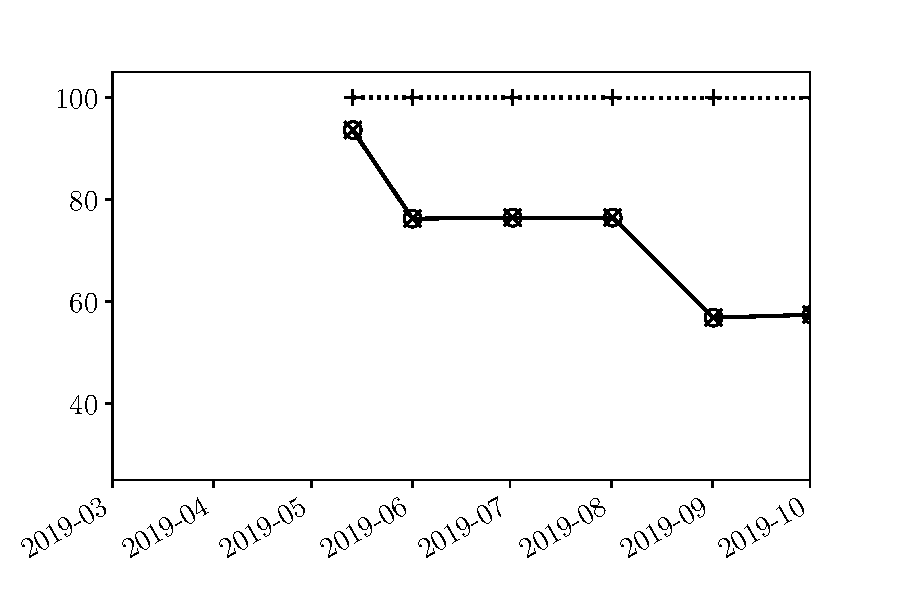
\includegraphics[width=0.5\textwidth]{figures/fig2a.pdf}}%
\subfigure[DataONE]{%
\label{fig:network-reliability-b}%
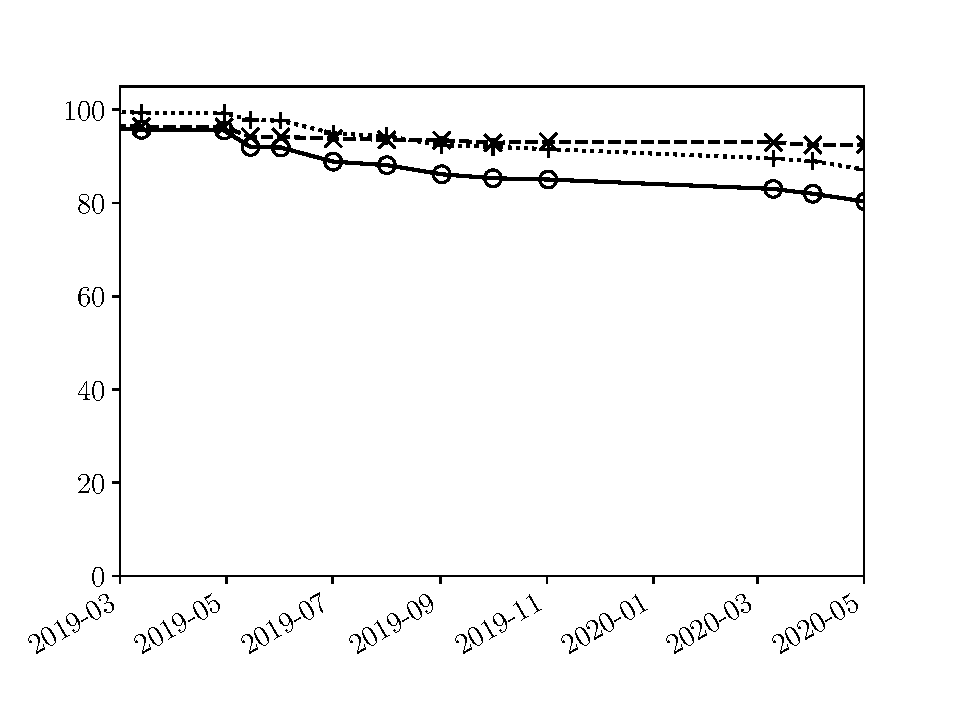
\includegraphics[width=0.5\textwidth]{figures/fig2b.pdf}} \\
\subfigure[GBIF]{%
\label{fig:network-reliability-c}%
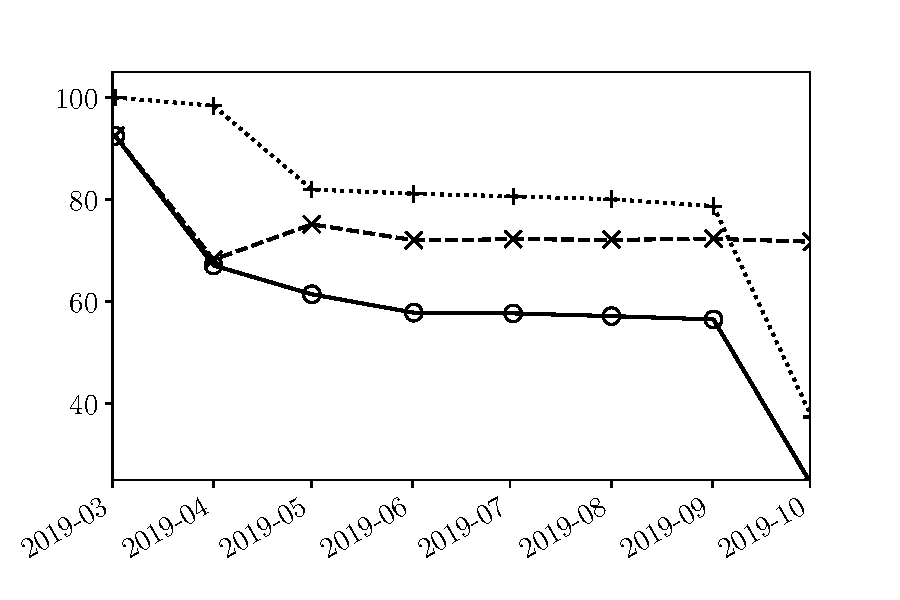
\includegraphics[width=0.5\textwidth]{figures/fig2c.pdf}}%
\subfigure[iDigBio]{%
\label{fig:network-reliability-d}%
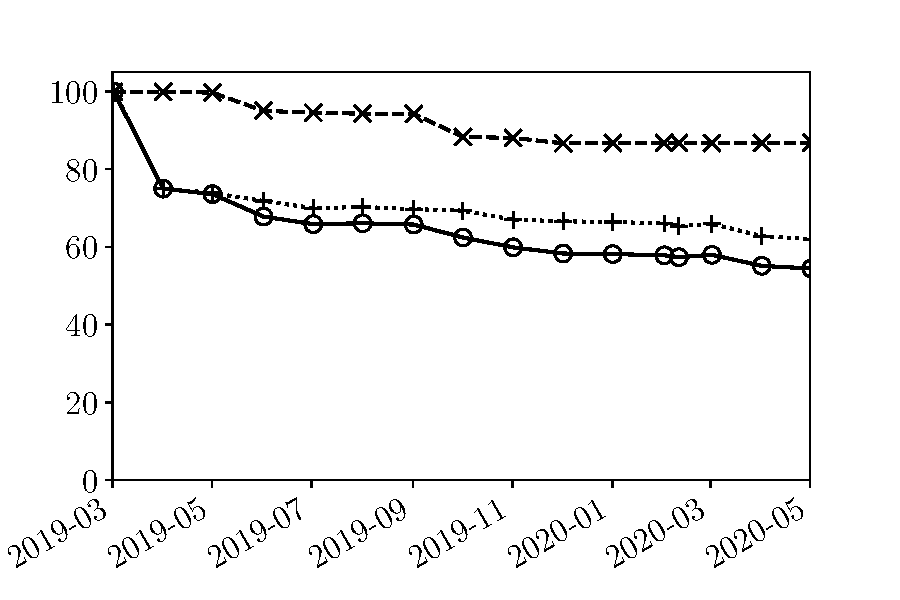
\includegraphics[width=0.5\textwidth]{figures/fig2d.pdf}} \\
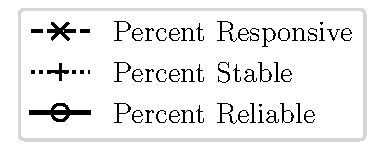
\includegraphics[scale=0.6]{figures/fig2legend.pdf}%

\caption[Network URL characteristics over time]{Overall responsiveness, stability, and reliability from March 2019 through May 2020 as percentages of URLs that exhibit each indicator in the provider networks of \subref{fig:network-reliability-a} BHL, \subref{fig:network-reliability-b} DataONE, \subref{fig:network-reliability-c} GBIF, and \subref{fig:network-reliability-d} iDigBio.
}%

\label{fig:network-reliability} % \label works only AFTER \caption within figure environment

\end{figure}

